\documentclass[tikz,border=10pt]{standalone}
\usepackage{tikz}
\usetikzlibrary{shapes.geometric, arrows, positioning}
\begin{document}
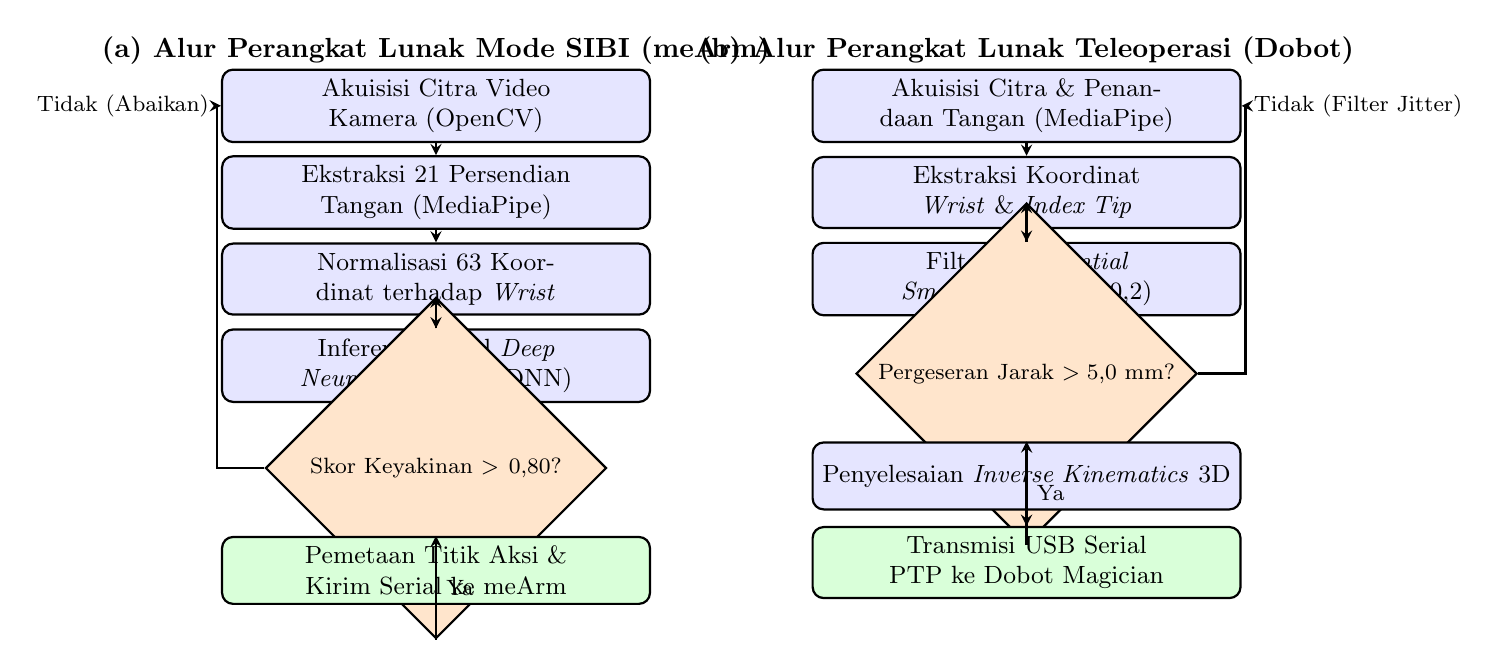
\begin{tikzpicture}[
    node distance=1.1cm,
    font=\small,
    box/.style={rectangle, draw=black, rounded corners, fill=blue!10, text centered, minimum height=0.85cm, text width=5.2cm, line width=0.8pt},
    decision/.style={diamond, draw=black, fill=orange!20, text centered, inner sep=2pt, line width=0.8pt, text width=3.8cm, font=\footnotesize},
    arrow/.style={thick, ->, >=stealth}
]
    % SIBI Pipeline (Left)
    \node at (0, 0.7) [font=\bfseries\normalsize] {(a) Alur Perangkat Lunak Mode SIBI (meArm)};
    \node (s1) [box] at (0, 0) {Akuisisi Citra Video Kamera (OpenCV)};
    \node (s2) [box, below of=s1] {Ekstraksi 21 Persendian Tangan (MediaPipe)};
    \node (s3) [box, below of=s2] {Normalisasi 63 Koordinat terhadap \textit{Wrist}};
    \node (s4) [box, below of=s3] {Inferensi Model \textit{Deep Neural Networks} (DNN)};
    \node (s5) [decision, below of=s4, yshift=-0.2cm] {Skor Keyakinan $> 0{,}80$?};
    \node (s6) [box, below of=s5, yshift=-0.2cm, fill=green!15] {Pemetaan Titik Aksi \& Kirim Serial ke meArm};
    
    \draw [arrow] (s1) -- (s2);
    \draw [arrow] (s2) -- (s3);
    \draw [arrow] (s3) -- (s4);
    \draw [arrow] (s4) -- (s5);
    \draw [arrow] (s5) -- node[right, font=\footnotesize] {Ya} (s6);
    \draw [arrow] (s5.west) -- ++(-0.6,0) |- node[near end, left, font=\footnotesize] {Tidak (Abaikan)} (s1.west);

    % Teleoperation Pipeline (Right)
    \node at (7.5, 0.7) [font=\bfseries\normalsize] {(b) Alur Perangkat Lunak Teleoperasi (Dobot)};
    \node (t1) [box] at (7.5, 0) {Akuisisi Citra \& Penandaan Tangan (MediaPipe)};
    \node (t2) [box, below of=t1] {Ekstraksi Koordinat \textit{Wrist} \& \textit{Index Tip}};
    \node (t3) [box, below of=t2] {Filter \textit{Exponential Smoothing} ($\alpha = 0{,}2$)};
    \node (t4) [decision, below of=t3, yshift=-0.1cm] {Pergeseran Jarak $> 5{,}0$ mm?};
    \node (t5) [box, below of=t4, yshift=-0.2cm] {Penyelesaian \textit{Inverse Kinematics} 3D};
    \node (t6) [box, below of=t5, fill=green!15] {Transmisi USB Serial PTP ke Dobot Magician};

    \draw [arrow] (t1) -- (t2);
    \draw [arrow] (t2) -- (t3);
    \draw [arrow] (t3) -- (t4);
    \draw [arrow] (t4) -- node[right, font=\footnotesize] {Ya} (t5);
    \draw [arrow] (t5) -- (t6);
    \draw [arrow] (t4.east) -- ++(0.6,0) |- node[near end, right, font=\footnotesize] {Tidak (Filter Jitter)} (t1.east);

\end{tikzpicture}
\end{document}
